\documentclass[class=report, crop=false, 12pt,a4paper]{standalone}
\usepackage{enumitem}
\usepackage{tikz}
\usepackage{float}
\usepackage{graphicx}
\usepackage{multicol}
\usepackage{siunitx}
\usepackage{mathtools}
\usepackage{amsmath}
\usepackage{amssymb}
\usepackage{commath}
\usepackage[normalem]{ulem}
\usepackage[a4paper,width=150mm,top=25mm,bottom=25mm]{geometry}
\begin{document}
\begin{center}
  26/10/2020
\end{center}
\textbf{Displacement measurements:}
\begin{itemize}
  \item Most frequent in manufacturing and process-control applications
  \item Work as a secondary transduction process in many transducers for other measurements such as force, torque, pressure, flow and density.
  \item Mostly requires a stationary reference point.
  \item Utilises a wide variety of techniques and principles.
\end{itemize}
\begin{figure}[H]
  \centering
  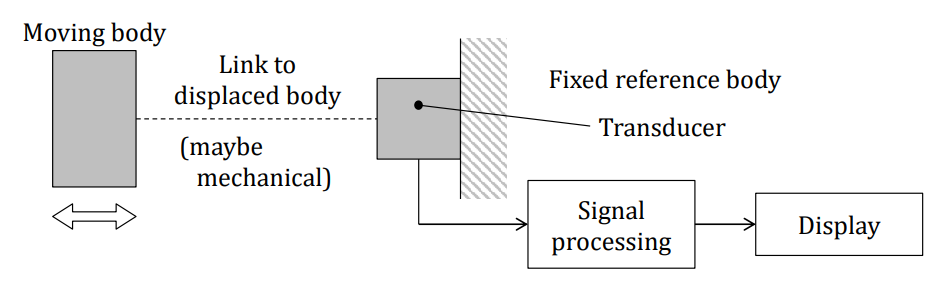
\includegraphics[width = 0.8 \textwidth]{../img/Mdiagram1.PNG}
\end{figure}
\section{Capacitance-Based Displacement Transducers}
\subsection{Capacitive Displacement Transducers}
Displacement changes the capacitance of the transducer. The capacitance of a parallel-plate capacitor is given by:
\begin{gather}
  C = \frac{\epsilon_0A}{d}
\end{gather}
Where:
\begin{itemize}
  \item $A$ is the area of the plates
  \item $d$ is the separation between the plates
  \item $\epsilon_0$ is the permittivity of free space $(8.854 \cdot 10^{-12}4 Fm^{-1})$
\end{itemize}
Example: The capacitance of the two metal cylinders is proportional to the area of overlap.
\begin{figure}[H]
  \centering
  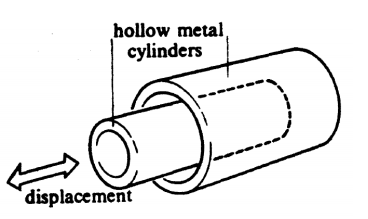
\includegraphics[width = 0.5 \textwidth]{../img/Mdiagram2.PNG}
\end{figure}
Variable capacitance can be introduced by an insulator between the plates. If the insulation is as thick as the plate separation, the overall capacitance is:
\begin{gather}
  C = \frac{\epsilon_0A_1}{d} + \frac{\epsilon_0\epsilon_rA_2}{d}
\end{gather}
Where:
\begin{itemize}
  \item $\epsilon_r$ is the relative permittivity of the insulator, or dialecetric as it is commonly known.
\end{itemize}
\begin{figure}[H]
  \centering
  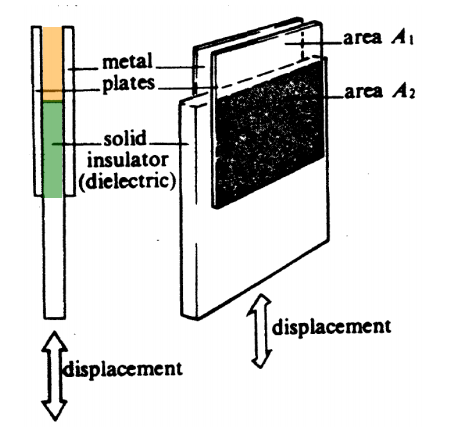
\includegraphics[width = 0.45 \textwidth]{../img/Mdiagram3.PNG}
  \caption{The orange part of the figure represents the 1st bit of the capacitance equation, when no insulator is inserted. The green part of the figure shows the 2nd part of the equation, where an insulator is introduced}
\end{figure}
\subsection{Measurement of Capacitance}
Suppose the capacitance of a capacitive transducer is a function of a displacement. When a constant voltage v is applied, charge is given as:
\begin{gather}
  q = Cv \\
  C = f(x) = \frac{q}{v}
\end{gather}
It is impossible to measure $q$ without disturbing it. If however, the voltage is made to vary, then $q$ must vary too, and its rate of change, current $i$, can be measured:
\begin{gather}
  \frac{\dif q}{\dif t}\left[\frac{C}{s}\right] = i[A]
\end{gather}
Differentiating $q = Cv$ with respect to time gives:
\begin{gather}
  \frac{\dif q}{\dif t} = i = C\frac{\dif v}{\dif t}
\end{gather}
If the applied voltage is sinusoidal, i.e. $v = V_0sin(\omega t)$, then:
\begin{gather}
  i = C\frac{\dif v}{\dif t} = V_0\omega cos(\omega t)
\end{gather}
The amplitude of the current, $i$, equals to $V_0\omega C$ (proportional to the capacitance). \\\\
Changes in capacitance caused by changes in displacement can be measured by determining the AC current flowing through the capacitor. However, in some cases in practice, the capacitance change due to the displacement is only a small fraction of the total capacitance and difficult to be measured:
\begin{gather}
  C_{total} = C_{transducer}+C_{cable}+C_{stray}
\end{gather}
\subsection{Differential Capacitance Displacement Transducers}
One way to get around the problem is to use either one of the differential forms of variable-separation or variable-area type transducer.
\begin{figure}[H]
  \centering
  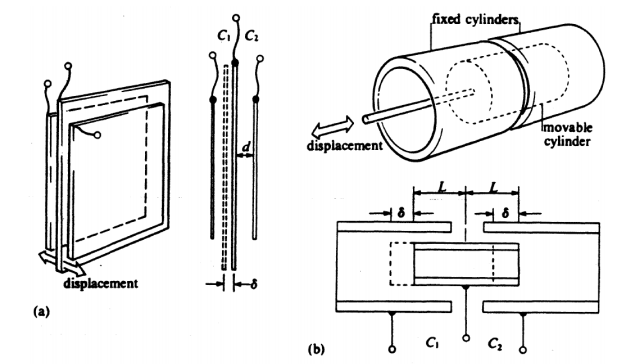
\includegraphics[width = 0.6 \textwidth]{../img/Mdiagram4.PNG}
\end{figure}
In each of the cases, two capacitors are formed which have equal capacitances when the transducer is geometrically centred.
\subsection{Capacitive Bridge}
The two capacitors are connected to a capacitive bridge. Here, difference in capacitance caused by the displacement unbalances the bridge and an AC output voltage $V_o$ occurs.
\begin{figure}[H]
  \centering
  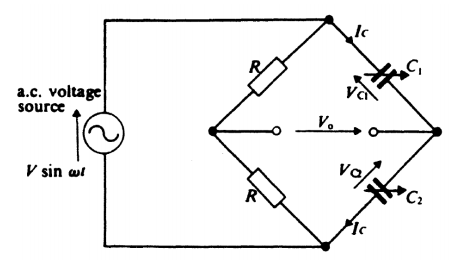
\includegraphics[width = 0.6 \textwidth]{../img/Mdiagram5.PNG}
\end{figure}
To derive $V_o$, we start with the voltages across each capacitor:
\begin{gather}
  V_{C1} = \frac{I_C}{\omega C_1} \\
  V_{C2} = \frac{I_C}{\omega C_2}
\end{gather}
This is because, if we consider voltage and currenct across/through a capacitor to be $v_C = V_Csin(\omega t)$ and $i_C = I_Ccos(\omega t)$,
\begin{gather}
  i_C = I_Ccos(\omega t) = C\frac{\dif v_C}{\dif t} = C\frac{\dif(V_Csin(\omega t))}{\dif t} = \omega CV_Ccos(\omega t) \\
  \therefore V_C = \frac{I_C}{\omega C}
\end{gather}
Now, knowing the voltages across each capacitor $V_{C1}$ and $V_{C2}$, the voltage across C2 as a fraction of the bridge energising voltage, V is:
\begin{gather}
  \frac{V_{C2}}{V} = \frac{V_{C2}}{V_{C1}+V_{C2}} \\
  = \frac{\frac{I_C}{\omega C_2}}{\frac{I_C}{\omega C_1}+\frac{I_C}{\omega C_2}} \\
  = \frac{C_1}{C_1+C_2}
\end{gather}
In the variable-separation type, the capacitances must be equal if the plate is centred. If the balance capacitance is $C_0$, then:
\begin{gather}
  C_0 = \frac{\epsilon_0A}{d}
\end{gather}
where $d$ is the balance separation. When the plate is displaced by a distance $\delta$ to the left as in the figure, we have:
\begin{figure}[H]
  \centering
  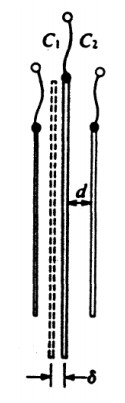
\includegraphics[width = 0.15 \textwidth]{../img/Mdiagram6.PNG}
\end{figure}
\begin{gather}
  C_1 = \frac{\epsilon_0A}{d-\delta} = C_0\frac{d}{d-\delta} \\
  C_2 = C_0\frac{d}{d+\delta}
\end{gather}
Substituting these for the equation of the voltage across $C_2$ yields:
\begin{gather}
  \frac{V_{C2}}{V} = \frac{d+\delta}{(d-\delta)+(d+\delta)} = \frac{d+\delta}{2d}
\end{gather}
The voltage across each resistor is half the energising voltage, so the amplitude of the output voltage is:
\begin{gather}
  V_o = V_{C2}-\frac{1}{2}V = \left(\frac{d+\delta}{2d}-\frac{1}{2}\right)V = \frac{\delta V}{2d}
\end{gather}
There is a linear relationship between the voltage output and the displacement, despite the non-linear capacitance–displacement relationship. \\\\
For the variable-area type, the capacitances are proportional to their active areas, so if the movable cylinder is displaced to the left, we have:
\begin{figure}[H]
  \centering
  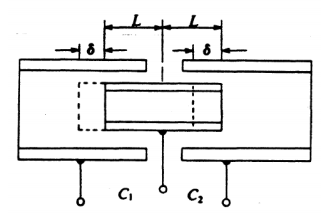
\includegraphics[width = 0.5 \textwidth]{../img/Mdiagram7.PNG}
\end{figure}
\begin{gather}
  C_1 = \frac{L+\delta}{L}C_0 \\
  C_2 = \frac{L-\delta}{L}C_0
\end{gather}
Substituting these for the equation of the voltage across $C_2$ yields:
\begin{gather}
  V_o = V_{C2}-\frac{1}{2}V = \frac{\delta V}{2L}
\end{gather}
In both cases, the output voltage can be expressed as:
\begin{gather}
  V_o = \frac{1}{2}xV
\end{gather}
\section{Inductance-Based Displacement Transducers}
\subsection{Linear Variable Differential Transformer (LVDT)}
\begin{figure}[H]
  \centering
  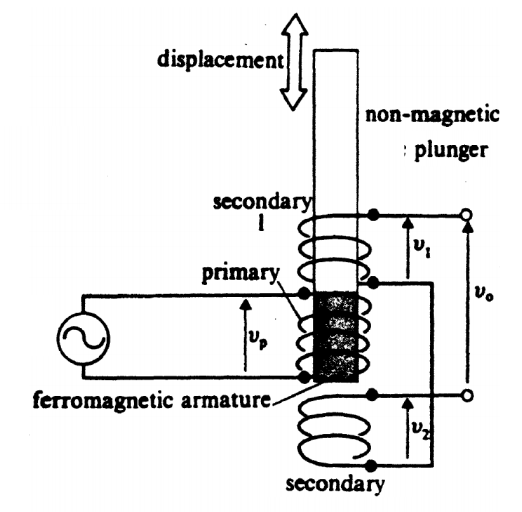
\includegraphics[width = 0.5 \textwidth]{../img/Mdiagram8.PNG}
\end{figure}
LVDT is one of the magnetic displacement transducers. An LVDT consists of:
\begin{itemize}
  \item Primary coil
  \item Two secondary coils
  \item Ferromagnetic armature (iron core)
  \item An AC energising source
  \item Non-magnetic plunger
  \item and AC voltages are induced in the secondary coil by transformer action.
\end{itemize}
\begin{figure}[H]
  \centering
  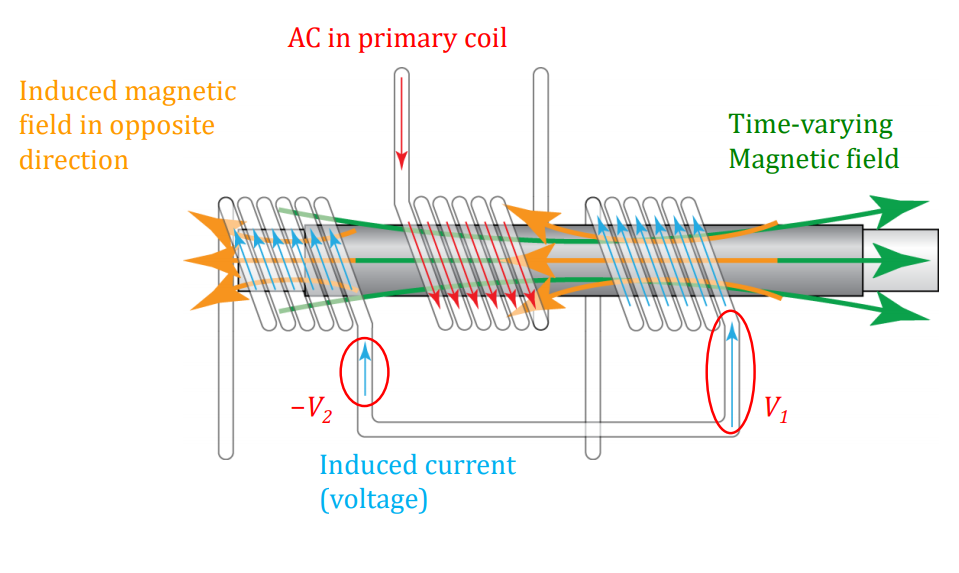
\includegraphics[width = 0.85 \textwidth]{../img/Mdiagram9.PNG}
  \caption{The working principle (with displacement to the right) of LVDTs}
\end{figure}
The working principle follows these steps:
\begin{enumerate}
  \item AC in primary coil
  \item Time-varying magnetic field
  \item Induced magnetic field in opposite
  \item Induced current (voltage)
\end{enumerate}
If there is no displacement, the output voltage will be 0. When a displacement occurs, the electro-magnetic field around one of the secondary coils (the one the ferromagnetic core moves towards) will be stronger. Hence, the induced current and voltage on that coil will be larger than the other one. 
\begin{gather}
  V_o = V_1-V_2 \neq 0 \rightarrow \propto displacement
\end{gather}
The postivie of negative value of $V_0$ can indicate the displacement of the core.
\begin{itemize}
  \item $V_o>0 \longrightarrow$ Displacement to right
  \item $V_o<0 \longrightarrow$ Displacement to left
\end{itemize}
\section{Resistance-Based Displacement Transducers}
A very common and simple form of displacement transducer.
\begin{figure}[H]
  \centering
  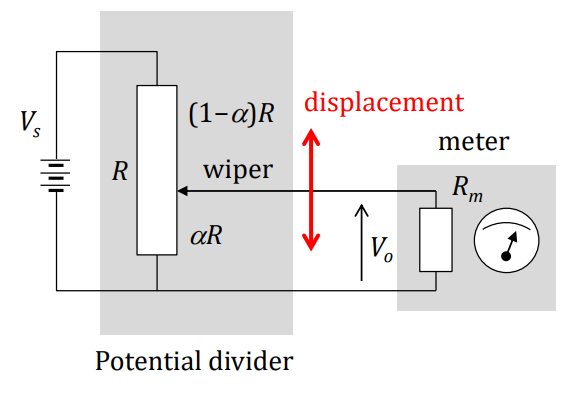
\includegraphics[width = 0.55 \textwidth]{../img/Mdiagram10.PNG}
\end{figure}
Resistor is typically a \textbf{coil winding}. Wiper displacement $\rightarrow$ change of $\alpha \ (0<\alpha<1)$. We assume the pot is wound uniformly with resistance wire and $\alpha$ varies linearly with the position of the wiper. With the internal resistance of the meter, the effective resistance $R_{eff}$ to determine $V_o$ is given as:
\begin{gather}
  R_{eff} = \alpha R || R_m = \frac{\alpha RR_m}{\alpha R+R_m}
\end{gather}
The two vertical lines $||$ indicate that $\alpha R$ and $R_m$ are in parallel. Using potential divider theory, the meter voltage $V_o$ is then:
\begin{gather}
  V_o = \frac{R_{eff}}{(1-\alpha)R+R_{eff}}V_s \\
  \frac{V_o}{V_s} = \frac{\alpha}{1+\alpha(1-\alpha)\frac{R}{R_m}}
\end{gather}
\begin{figure}[H]
  \centering
  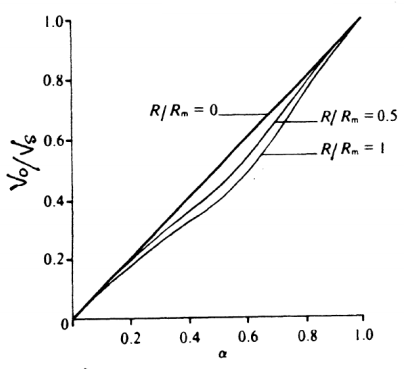
\includegraphics[width = 0.55 \textwidth]{../img/Mdiagram11.PNG}
\end{figure}
\begin{itemize}
  \item If $R_m>>R$, then $\frac{V_o}{V_s}$ is approximated as linear.
  \item If $R_m>10R$, then the maximum error is approximated as $Err_{max} = 15\frac{R}{R_m}(\%)$
\end{itemize}
Increasing $V_s$ will increase the sensitivity (= $V_o$ / wiper travelling distance), but it also increases the power dissipated by the pot.
\begin{gather}
  P = \frac{V_s^2}{R} \longrightarrow V_{s,max} = \sqrt{P_{max}R}
\end{gather}
$P_{max}$ is the rated maximum power dissipation (given in spec sheet). To increase the spatial resolution of pot:
\begin{itemize}
  \item carbon film
  \item conductive plastic
  \item ceramic-metal mix
\end{itemize}
could also be used. These also reduce the friction between the wiper and the resistive element. Linear resistance pots are made with spans ranging from about 10 mm to almost 1m.
\section{Measuring Rotational Displacement}
\subsection{Optical Incremental Shaft Encoder}
The output signals here, i.e. voltage output from the photosensor, depend on the angular displacement of the shaft.
\begin{figure}[H]
  \centering
  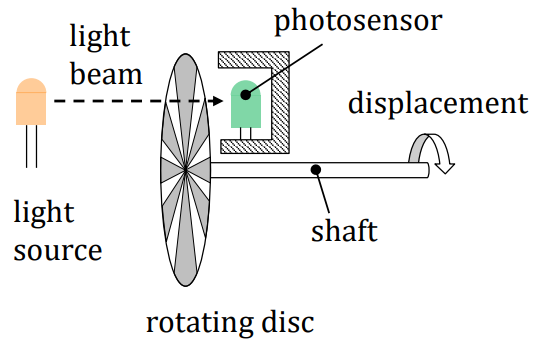
\includegraphics[width = 0.6 \textwidth]{../img/Mdiagram12.PNG}
\end{figure}
The pattern of the grating allow/disallow the light to reach the photosensor. The signal output varies depending on the \textbf{relative position} of the grating. Sinusoidal signal outputs are expected. \\\\
More elaborated version of incremental shaft encoder includes one with two discs (Moiré fringes) and two sensors.
\begin{figure}[H]
  \centering
  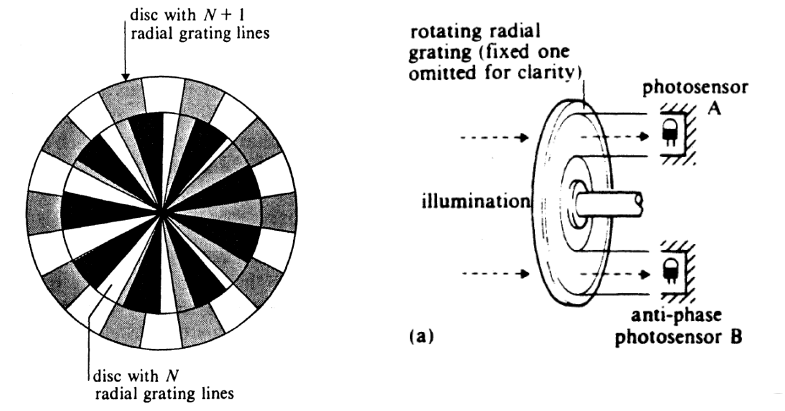
\includegraphics[width = 0.7 \textwidth]{../img/Mdiagram13.PNG}
\end{figure}
Differential output can be taken for clear signal.
\begin{figure}[H]
  \centering
  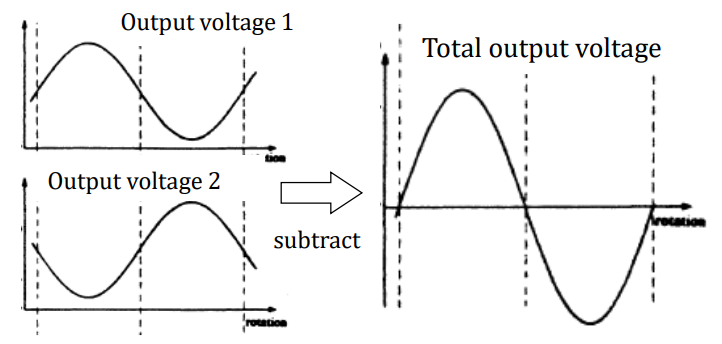
\includegraphics[width = 0.75 \textwidth]{../img/Mdiagram14.PNG}
\end{figure}
Advantage of the differential systems:
\begin{itemize}
  \item Reduced influence by light variability
  \item Reduced influence by the environment
\end{itemize}
\begin{figure}[H]
  \centering
  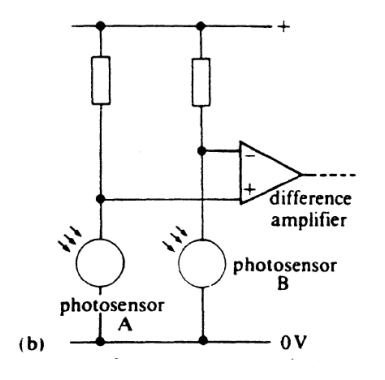
\includegraphics[width = 0.45 \textwidth]{../img/Mdiagram15.PNG}
\end{figure}
The pairs of light source and sensor may be placed 90\si{\degree} apart, in order to sense the direction of rotation .
\begin{figure}[H]
  \centering
  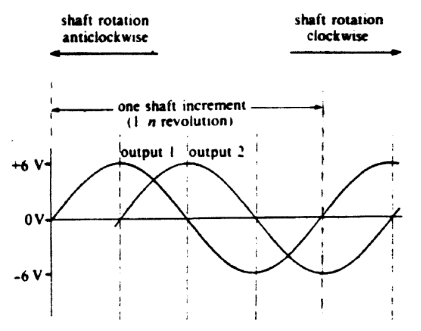
\includegraphics[width = 0.55 \textwidth]{../img/Mdiagram16.PNG}
\end{figure}
\subsection{Optical Absolute Shaft Encoder}
Similar mechanism can be used as to measure an \textbf{absolute} rotary displacement by using binary code on the disc.
\begin{figure}[H]
  \centering
  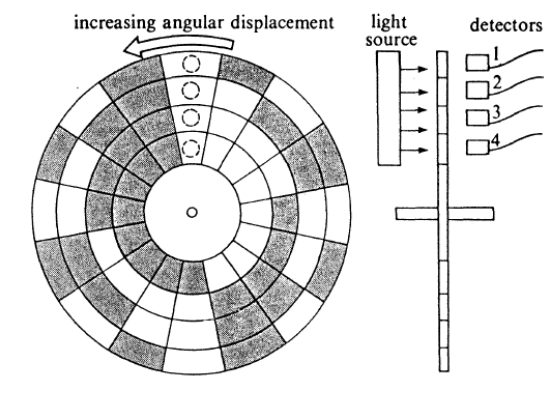
\includegraphics[width = 0.55 \textwidth]{../img/Mdiagram17.PNG}
\end{figure}
The four track disc above can have $2^4 = 16$ patterns $\longrightarrow$ 16 segments around the disc (resolution: $\frac{360}{16} = 22.5$\si{\degree}). In general, the resolution is:
\begin{gather}
  \frac{360}{2^{\ number \ of \ tracks}}(\si{\degree})
\end{gather}
and the detector output ranges from 0 to $2^{(number \ of \ tracks)}-1$.
\section{Measuring Large Linear Displacement}
\subsection{Measurement of Large Linear Displacements}
The linear displacement transducers studied so far measure displacements of up to 1m. In order to measure larger displacements, other method are used. The simplest form of these is:
\begin{figure}[H]
  \centering
  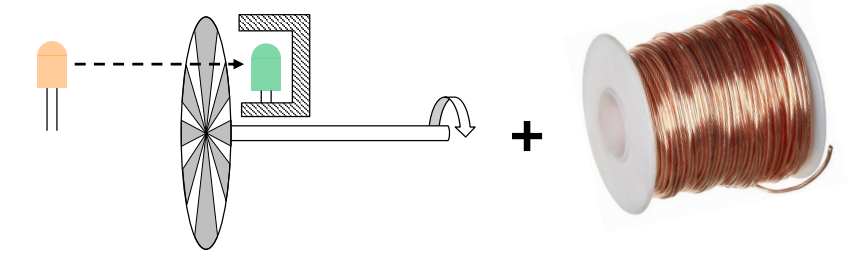
\includegraphics[width = 0.85 \textwidth]{../img/Mdiagram18.PNG}
\end{figure}
Commercial transducers of this type are available for displacements ranging from 50 mm to over 50m.
\subsection{Wave Propagation Methods}
Non-contact displacement measurements over long distances are possible by using ultrasonic waves, radio waves and light waves.
\subsubsection{Pulse Reflection (Time of Flight)}
\begin{figure}[H]
  \centering
  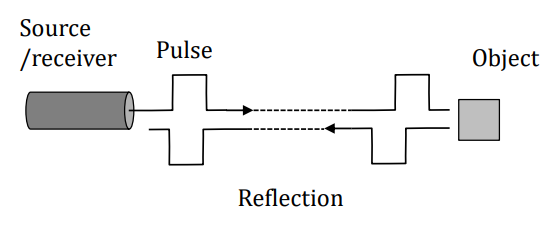
\includegraphics[width = 0.75 \textwidth]{../img/Mdiagram19.PNG}
\end{figure}
\begin{gather}
  D = V_{wave} \cdot \Delta t
\end{gather}
Type of the pulse:
\begin{itemize}
  \item Sonic/ultrasonic - $330$ \si{\metre\per\second} (in the air)
  \item Radio/light wave - $3\cdot 10^8$ \si{\metre\per\second}
\end{itemize}
\textbf{Accuracy of the measurement hinges on the measurement accuracy of time.} \\\\
Other points to be considered:
\begin{itemize}
  \item What is the medium
  \item Obstacles in the middle
  \item Diffraction
  \item ...
\end{itemize}
\subsubsection{Phase Measurement}
A continuous radio wave is emitted instead of pulses. The phase difference between the transmitted sine wave and the reflected sine wave is used to measure displacement.
\begin{figure}[H]
  \centering
  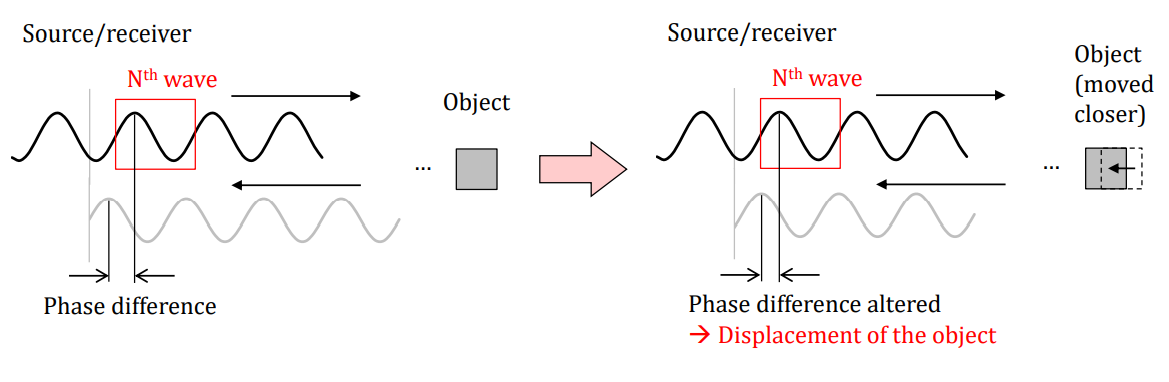
\includegraphics[width = 1 \textwidth]{../img/Mdiagram20.PNG}
\end{figure}
\subsubsection{Some Examples of Laser Distance Measurement}
\textbf{Laser range finders}
\begin{itemize}
  \item Distance: 15-400 m
  \item Error: 0.1\% at 1 m
\end{itemize}
\textbf{Laser scanner for 3D modelling}
\begin{itemize}
  \item Scan a 3D object with 4 lasers at about 127 $\mu m$ accuracy to obtain its surface coordinates (used with tranangulation).
\end{itemize}
\section{Other Methods of Measuring Position and/or Displacement}
\subsection{Projection Mapping}
\begin{itemize}
  \item Working principle of object/motion detection in Microsoft Kinect
  \item Detects objects shape or motion
  \item The projection from a light source is projected onto the object, and a number of cameras are used to detect and capture the image, based on the angle difference of the captured images.
  \item Applicable Range: 1.2-3.5 m (50 cm to 5 m)
  \item Depth Resolution: 
\end{itemize}
\subsection{Global Positioning System (GPS)}
Location service with GPS
\begin{figure}[H]
  \centering
  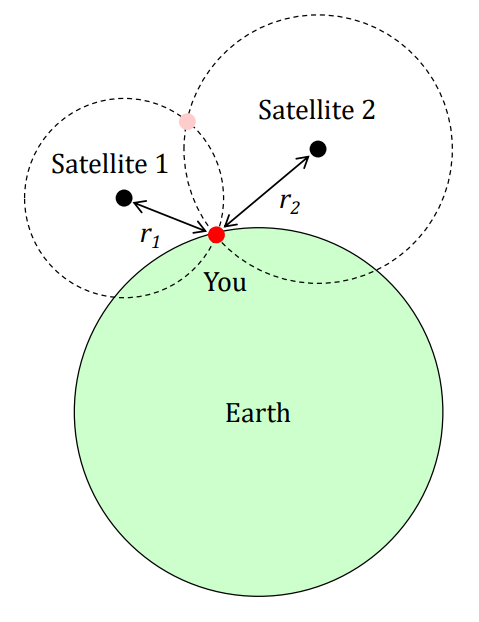
\includegraphics[width = 0.35 \textwidth]{../img/Mdiagram21.PNG}
\end{figure}
The distances between GPS satelites, $r_1$ and $r_2$, are measured by time of flight of radio waves. The location of the person $(x,y,z)$ is determined by solving:
\begin{gather}
  r_i^2 = (X_i-x)^2+(Y_i-y)^2+(Z_i-z)^2
\end{gather}
with known locations of the satelites $(X,Y,Z)$. To identify the position in 3D, 3 equations are needed, i.e. you need to communicate with 3 satellites.
\section{Datasheet}
Datasheets are documents providing the specifications for a particular product. Some relevant examples from datasheets are:
\begin{itemize}
  \item \textbf{Linearity:} how much the voltage-displacement relationship could go off the linear.
  \item \textbf{Temperature coefficient of sensitivity:} change of sensitivity due to the operating temperature
  \item \textbf{Zero shift with temperature:} how much the null position (location) could be shifted due to the operating temperature
  \item \textbf{Output ripple:} ‘Hint’ of AC input in DC output. Does not affect the mean DC output value.
  \item \textbf{Resistance range:} Range of available (total) pot resistance
  \item \textbf{Output smoothness:} Maximum resolution error
  \item \textbf{Tolerance:} Uncertainty in manufacturing of the resistance element
\end{itemize}
\end{document}